\section[Input Amplifier Level]{\textit{Input Amplifier Level}}
\sectionmark{\textit{Input Amplifier Level}}

Este módulo, compuesto únicamente por 8 diales de ganancia (Ver \ref{fig:input_amplifier_level}), controla los 8 canales de entrada del Synthi 100\footnote{En total son 16 las entradas si contamos, además de los 8 \textit{Input Amplifier Level}, las 4 entradas de retorno desde otros dispositivos y los 2 canales específicos para micrófonos.}. No sin cierta simetría, este es el mismo número de canales que tiene para la salida de audio. 

\begin{figure}
	\centering
	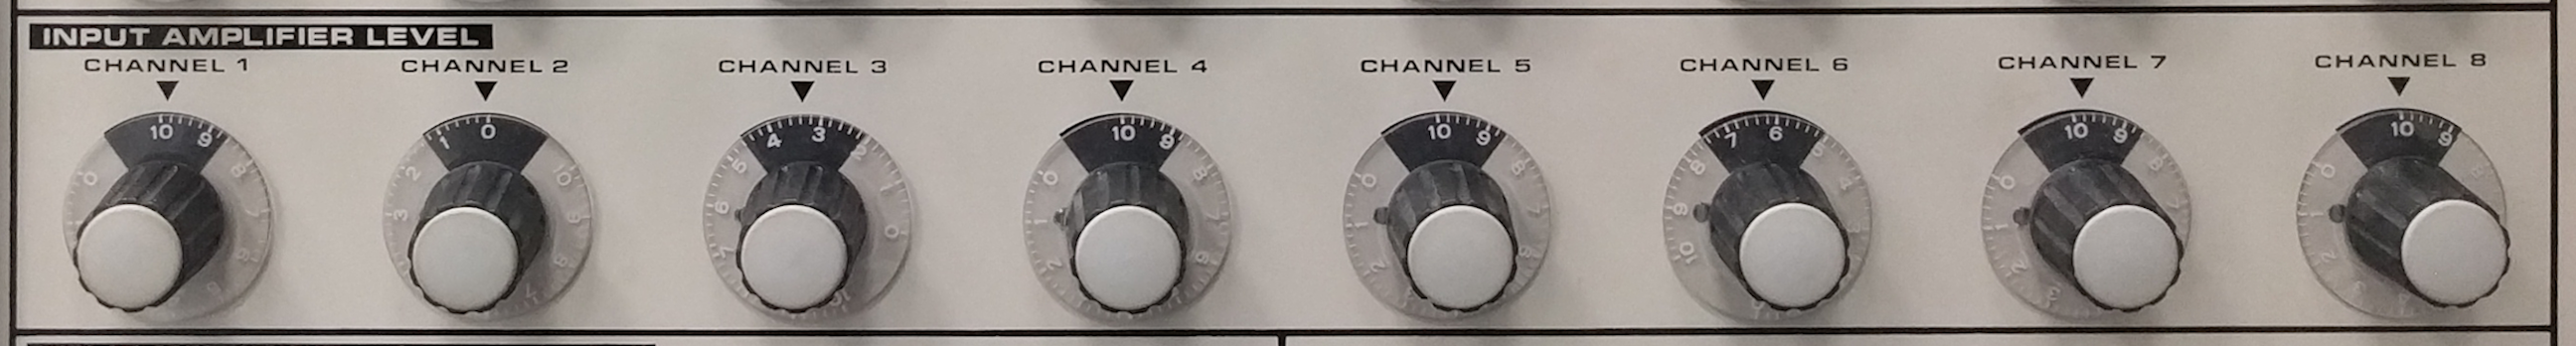
\includegraphics[width=1\textwidth]{images/input_amplifier_level}
	\caption[\textit{Input Amplifier Level}]{\textit{Array} de las ganancias de los 8 canales de entrada}
	\label{fig:input_amplifier_level}
\end{figure}

Las señales que por estos canales se reciben son ambivalentes, pudiendo ser tanto de audio como de voltaje, con lo que son conectables con cualquiera de las entradas de cualquier módulo del sintetizador. Esta característica hace el sintetizador modular un módulo en sí mismo capaz de ser controlado por cualquier señal exterior. 